In order to compare this paper's best configuration's performance with the one found in 
paper \cite{peter},
each best configuration is set to play 50 games 1000 times. 
Since this paper's best configuration already 
is found to be normally distributed in its average win rate, the comparative paper's best 
configuration is tested resulting in the qq-plot shown in figure~\ref{fig:peter-qq-plot}.
\begin{figure}
	\begin{small}
		\begin{center}
			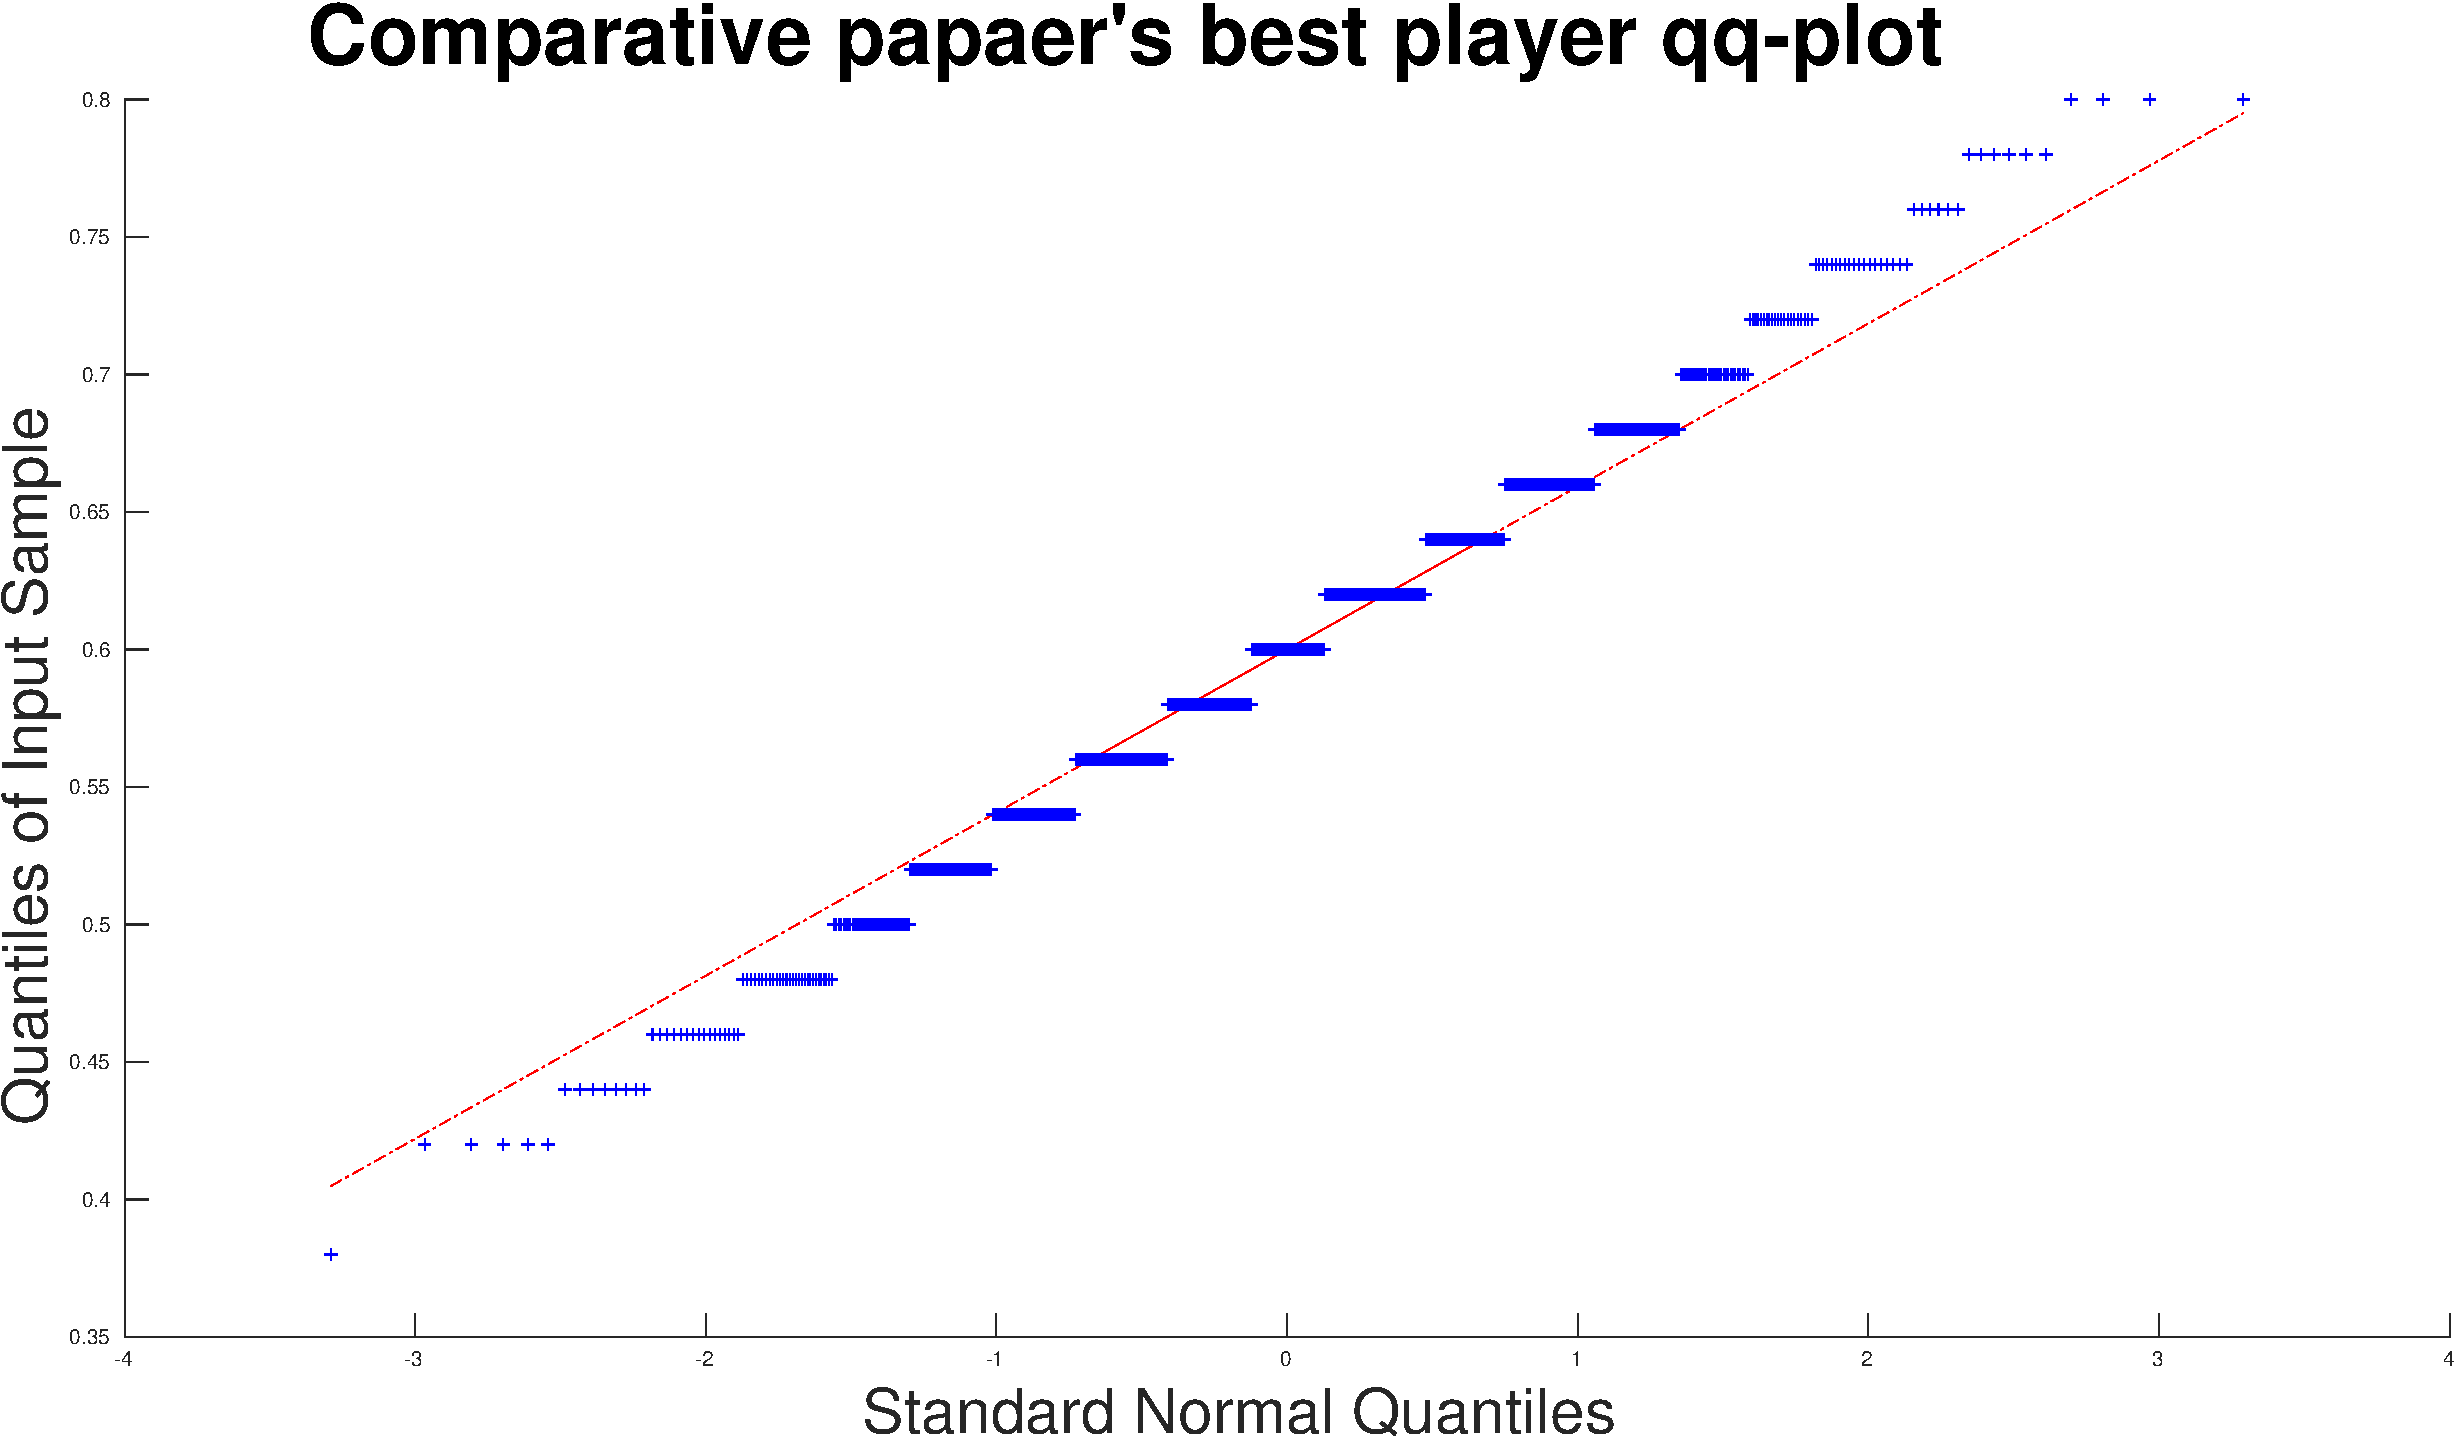
\includegraphics[width=0.9\textwidth]{fig/peter-qq-plot.pdf}
		\end{center}
		\caption{qq-plot of the comparative paper's best configuration win rate over 50 games 1000 times}
		\label{fig:peter-qq-plot}
	\end{small}
\end{figure}
Based on the found qq-plot it is concluded that the comparative paper's configuration 
data are sufficiently normality distributed. A Bartlett test is then performed to test for equal variance. 
Here a p-value of $0.52$ is found, and thus it is assumed that the samples have equal variance. 
All the necessary criteria has now been fulfilled to perform a 2 sample t-test to assert
if there is statistical evidence to support that the two configurations are from different underlying 
normal distributions.
Here a p-value of approximately $ 2.9\cdot 10^{-17}$ is found, 
and thus the samples are not of the same distribution. Finally to determine which configuration 
performs the best, the mean is found for each algorithm as shown in table~\ref{tab:final-result}
\begin{table}[H]
	\begin{center}
		\caption{Means of C3 and the best configuration from the comparative paper}
		\label{tab:final-result}
		\begin{tabular}{|l|l|}
			\hline
			{}					& Mean   \\ \hline
			C3					& 0.583  \\ \hline
			Comparative paper 	& 0.609 \\ \hline
		\end{tabular}
	\end{center}
\end{table}
It can here be seen that the best configuration is produced by the comparative paper
with a mean avg win rate of $60.9\%$ compared to the one found in this paper at $58.3\%$.
The ranked lists of the two best configurations can be seen in table~\ref{tab:ranked-victor}
for this paper, and for the comparative paper in table~\ref{tab:ranked-peter}
\begin{table}[!htb]
    \begin{minipage}[b]{.5\linewidth}
		\centering
		\caption{The ranked actions from the chromosome of C3 from this paper}
		\label{tab:ranked-victor}
        \begin{tabular}[t]{|l|l|l|} \hline
			Ranking & Action & Value \\ \hline
			0  & \texttt{            MOVE\_FROM\_HOME }&  3.451 \\
			1  & \texttt{    MOVE\_ONTO\_ANOTHER\_DIE }&  1.098 \\
			2  & \texttt{                        MOVE }&  0.912 \\
			3  & \texttt{ MOVE\_ONTO\_GLOBE\_AND\_DIE }&  0.791 \\
			4  & \texttt{   MOVE\_ONTO\_VICTORY\_ROAD }&  0.789 \\
			5  & \texttt{ MOVE\_ONTO\_STAR\_AND\_KILL }&  0.394 \\
			6  & \texttt{            MOVE\_ONTO\_GOAL }&  0.193 \\
			7  & \texttt{           MOVE\_ONTO\_GLOBE }& -0.198 \\
			8  & \texttt{            MOVE\_ONTO\_STAR }& -0.389 \\
			9  & \texttt{ MOVE\_FROM\_HOME\_AND\_KILL }& -0.596 \\
			10 & \texttt{  MOVE\_ONTO\_STAR\_AND\_DIE }& -2.303 \\
			11 & \texttt{   MOVE\_ONTO\_ANOTHER\_KILL }& -5.480 \\ \hline
        \end{tabular}
    \end{minipage}%
	\hspace{0.3cm}
	\begin{minipage}[b]{.5\linewidth}
      \centering
	  \caption{The ranked actions from the chromosome of the best configuration from the comparative paper}
	  \label{tab:ranked-peter}
	  	\begin{tabular}[t]{|l|l|l|}\hline
			Ranking & Action & Value \\ 
			\hline
			0  & \texttt{MOVE\_FROM\_HOME\_AND\_KILL}&   237 \\
			1  & \texttt{MOVE\_ONTO\_GOAL}&              235 \\
			2  & \texttt{MOVE\_ONTO\_ANOTHER\_KILL}&     228 \\
			3  & \texttt{MOVE\_ONTO\_STAR\_AND\_DIE}&    181 \\
			4  & \texttt{MOVE\_ONTO\_STAR\_AND\_KILL}&   119 \\
			5  & \texttt{MOVE\_FROM\_HOME}&              97 \\
			6  & \texttt{MOVE\_ONTO\_STAR}&              95 \\
			7  & \texttt{MOVE\_ONTO\_VICTORY\_ROAD}&     93 \\
			8  & \texttt{MOVE\_ONTO\_GLOBE}&             86 \\
			9 & \texttt{MOVE}&                          83 \\
			10 & \texttt{MOVE\_ONTO\_ANOTHER\_DIE}&      65 \\
			11 & \texttt{MOVE\_ONTO\_GLOBE\_AND\_DIE}&   16 \\ 
			\hline
		\end{tabular}
	\end{minipage} 
\end{table}

When considering the shown difference in performance, the hyper parameters of interest 
include the generation size, the lower mutation rate, the selection method,
the chromosome representation and the use of elitism.\par
The generation size being 128 compared to the one used in this paper of 100, 
explains part of the difference in performance, since a wider search provides more 
opportunities for well performing solutions.
For a lower introduction of new genetic material, the comparative paper applies a
lower mutation rate of 1\%, which is less likely destroy useful genes.
Combined with the use of elitism, a greater emphasis is placed on conserving 
well performing genetic material.
The comparative paper uses a roulette selection method, which in this paper was demonstrated to 
provide inferior results compared to tournament selection. 
The possible downsides of roulette selection are likely 
mitigated by greater genetic preservation in the comparative paper. 
Another possibility could be that roulette selection does provide greater 
benefits with the comparative paper's other configurations, though based on 
the great similarity between the algorithms, this seems unlikely.\\
Possible improvements to the methods in this paper include 
a greater number of games to represent individual's performance and 
a more detailed action space representation.
Here 100 games would be a beneficial improvement from the 50 games used, 
and a more detailed action space representation \\ (e.g. \texttt{MOVE\_INTO\_DANGER})
would give more nuanced representation of the games current state.
However this would add significant computational complexity to the method, 
resulting in a large time penalty and require more computational 
resources than available for this project.
Finally while the mean avg win rates of the two configurations are 
relatively close, the actions rankings have very little overlap. How exactly
said overlap result in such similar avg win rates require further research.
